\chapter{Инфляция, обусловленная скатывающимся скалярным полем}

\lectureoverview{Вопрос, оставшийся с прошлой лекции, задает основное уравнение,
\(\ddot\phi+3H\dot\phi=-V'(\phi)\): что движется, что создает силу и почему расширение похоже на трение? Сначала мы выведем это уравнение в фиксированном объеме, а затем — в расширяющемся. В сочетании с уравнением Фридмана оно дает механизм медленного скатывания, при котором высокий, пологий потенциал скалярного поля вызывает почти экспоненциальное расширение. Инфляция разбавляет монополи и сглаживает геометрию; ее конец повторно нагревает Вселенную и запускает стандартную стадию горячего Большого взрыва. Тогда неизбежно возникает последняя проблема: если инфляция сглаживает так эффективно, откуда взялась структура? Одномерный расчет каустик показывает, как крошечные вариации скорости порождают слои, филаменты и узлы, оставляя квантовое происхождение этих вариаций до следующей лекции.}

\section{Что на что действует?}

Вопрос в начале лекции возвращает нас к уравнению
\begin{equation}
\ddot\phi+3H\dot\phi
=F(\phi)
=-\frac{dV}{d\phi}
\label{eq:c09-opening}
\end{equation}
и спрашивает, какая сила \(F\) может действовать на поле. Этот вопрос далеко не второстепенный. Чтобы ответить на него, мы должны восстановить механику поля и тем самым начинаем саму тему инфляции.

Скалярное поле сопоставляет каждой точке пространства и времени одно число \(\phi(\mathbf x,t)\). Электрическое и магнитное поля несут энергию; скалярное поле тоже может нести ее. Нужное нам здесь поле гипотетично: никакой конкретный инфлатон экспериментально не обнаружен, поэтому его энергия как функция значения поля неизвестна. Поэтому мы задаем его не заданной явно плотностью потенциальной энергии
\begin{equation}
V=V(\phi).
\label{eq:c09-potential}
\end{equation}
Разным значениям \(\phi\) соответствуют разные количества энергии, запасенной в единице физического объема.

Нет никаких оснований считать, что при \(\phi=0\) энергия равна нулю. Начало отсчета в пространстве поля — дело соглашения, особенно для еще не открытого поля, и сдвиг координаты, которой помечают значения поля, не обязан помещать минимум \(V\) в начало координат. График \(V(\phi)\) описывает относительные наклоны и высоты, а не какую-то выделенную исходную точку для поля.

Потенциальная энергия — это та часть, которая остается, когда поле в данный момент неподвижно. Если поле меняется со временем, у него есть и кинетическая энергия. Величина \(\dot\phi\) — не скорость объекта в обычном пространстве; это скорость, с которой меняется значение поля, то есть скорость в пространстве поля. Полезную аналогию дает упругая струна. Ее смещение является полем на одномерном мире, и колеблющийся элемент струны обладает кинетической энергией, пропорциональной квадрату производной этого смещения по времени.

Коэффициент при этом квадрате можно поглотить в определение поля. Если начать с
\begin{equation}
\frac12 n^2\dot\phi^{\,2},
\end{equation}
то замена переменной
\begin{equation}
\chi=n\phi
\end{equation}
превращает этот член в \(\dot\chi^{\,2}/2\). Поэтому мы можем выбрать канонически нормированное поле и записать в однородном приближении,
\begin{equation}
\rho_\phi=\frac12\dot\phi^{\,2}+V(\phi).
\label{eq:c09-rho-homogeneous}
\end{equation}
Этот выбор представляет собой нормировку координаты в пространстве поля, а не утверждение о том, что масса какой-то реальной частицы положена равной единице.

\section{Механика в фиксированном объеме}

Рассмотрим малый объем, в котором поле почти постоянно по пространству. Его плотность энергии имеет ту же математическую форму, что и энергия частицы единичной массы: кинетическая плюс потенциальная. Соответствующая плотность лагранжиана имеет противоположный знак при потенциальной энергии,
\begin{equation}
\mathcal L_\phi
=\frac12\dot\phi^{\,2}-V(\phi).
\label{eq:c09-lagrangian-density}
\end{equation}
Аналогия здесь математическая. Обобщенная координата — это значение поля, а не пространственное положение частицы.

Уравнение Эйлера--Лагранжа имеет вид
\begin{equation}
\frac{d}{dt}
\left(
\frac{\partial\mathcal L_\phi}{\partial\dot\phi}
\right)
=
\frac{\partial\mathcal L_\phi}{\partial\phi}.
\label{eq:c09-el-fixed}
\end{equation}
Здесь переменная скорости — \(\dot\phi\), поэтому
\begin{equation}
\frac{\partial\mathcal L_\phi}{\partial\dot\phi}=\dot\phi,
\qquad
\frac{\partial\mathcal L_\phi}{\partial\phi}=-V'(\phi),
\end{equation}
получаем
\begin{equation}
\ddot\phi=-V'(\phi)\equiv F(\phi).
\label{eq:c09-fixed-eom}
\end{equation}
Вторая производная — это ускорение полевой координаты, а отрицательный наклон потенциала — действующая на неё сила.

\begin{figure}[htbp]
\centering
\includegraphics[width=0.88\textwidth]{lecture_09_figure_03.png}
\caption{На читаемой части доски \(V(\phi)\) переходит в уравнение для фиксированного объёма \(\ddot\phi=-\partial V/\partial\phi\). Верхнее выражение Эйлера--Лагранжа частично обрезано и заслонено, поэтому уравнение~\eqref{eq:c09-el-fixed} восстановлено по выводу, а не приведено как полная запись с кадра.}
\label{fig:c09-fixed-board}
\lectureframe{00:10:53.836}
\end{figure}

\begin{classroomqa}
\audiencequestion{Что это за сила и на что она действует?}
\lecturerresponse{Эволюционирующей величиной является скалярное значение \(\phi\). Величина \(-V'(\phi)\) — это сила в пространстве поля: она ускоряет значение поля в сторону меньшей потенциальной энергии, так же как \(-dV/dx\) ускоряет координату частицы. Это не новая векторная сила, проталкивающая материальное тело через обычное пространство. \lecturetimestamp{00:00:27--00:00:49; 00:10:41--00:11:29}}
\end{classroomqa}

Полное поле может зависеть от пространственных координат. Для канонического скалярного поля в пространственно плоской расширяющейся геометрии его локальная плотность энергии содержит
\begin{equation}
\rho_\phi
=
\frac12\dot\phi^{\,2}
+\frac{1}{2a^2}\lvert\nabla\phi\rvert^2
+V(\phi).
\label{eq:c09-rho-full}
\end{equation}
Мы отбрасываем градиентный член, потому что расширение растягивает неоднородности до больших длин волн, делая поле почти однородным внутри малого объёма. Это приближение, оправданное космологической ситуацией, а не отрицание того, что скалярные волны или пространственные ряби могут существовать.

\section{Расширяющийся объём}

Первый вывод отвечает на исходный вопрос, но это ещё не космологический вывод. Уравнения~\eqref{eq:c09-rho-homogeneous} и \eqref{eq:c09-lagrangian-density} представляют собой плотности. Единичная сопутствующая ячейка имеет физический объём, пропорциональный \(a^3(t)\), поэтому её лагранжиан равен
\begin{equation}
L_\phi
=a^3(t)
\left[
\frac12\dot\phi^{\,2}-V(\phi)
\right].
\label{eq:c09-comoving-lagrangian}
\end{equation}
Множитель \(a^3\) был бы несущественным в статическом объёме. В космологии он зависит от времени, и именно эта зависимость даёт недостающий член.

\begin{figure}[htbp]
\centering
\includegraphics[width=0.88\textwidth]{lecture_09_figure_04.png}
\caption{Слева видна нарисованная от руки кривая потенциала, а справа — фрагменты выражений для энергии и лагранжиана. Кривая и смена знака надёжно читаются; полная алгебра в уравнении~\eqref{eq:c09-comoving-lagrangian} взята из устного вывода, поскольку лектор заслоняет часть доски.}
\label{fig:c09-potential-board}
\lectureframe{00:13:26.528}
\end{figure}

Применяя уравнение Эйлера--Лагранжа к \(L_\phi\), получаем
\begin{align}
\frac{d}{dt}\left(a^3\dot\phi\right)
&=-a^3V'(\phi), \label{eq:c09-a3-form}\\
a^3\ddot\phi+3a^2\dot a\,\dot\phi
&=-a^3V'(\phi),\\
\ddot\phi+3\frac{\dot a}{a}\dot\phi
&=-V'(\phi).
\end{align}
С учётом \(H=\dot a/a\) результат принимает вид
\begin{equation}
\boxed{\ddot\phi+3H\dot\phi=-V'(\phi)}.
\label{eq:c09-hubble-friction}
\end{equation}
Уравнение, которое вспоминалось в начале, теперь выведено, а не просто воспроизведено по памяти.

\begin{figure}[htbp]
\centering
\includegraphics[width=0.96\textwidth]{lecture_09_figure_05.png}
\caption{Слева — динамика в фиксированном объёме, справа — поправка для расширяющегося объёма. Видимая часть доски подтверждает последовательность от \(d(a^3\dot\phi)/dt\) к формам с \(3\dot a/a\) и \(3H\); обрезанные правые части дополняются уравнением~\eqref{eq:c09-a3-form}.}
\label{fig:c09-expanding-board}
\lectureframe{00:18:35.380}
\end{figure}

\begin{classroomqa}
\audiencequestion{Можно ли более наглядно представить силу \(F\)?}
\lecturerresponse{Изобразите \(V(\phi)\) как ландшафт, горизонтальная координата которого — значение поля. Наклон определяет силу, \(F=-V'(\phi)\). Крутой спуск вниз даёт большую движущую силу в пространстве поля; пологий — малую. Этот образ помогает представить одномерную полевую координату, а не буквальный холм, расположенный в физическом пространстве. \lecturetimestamp{00:18:26--00:19:18}}
\end{classroomqa}

\section{Хаббловское трение и установившееся движение}

Перенесём средний член в уравнении~\eqref{eq:c09-hubble-friction} вправо:
\begin{equation}
\ddot\phi=-V'(\phi)-3H\dot\phi.
\end{equation}
В расширяющейся Вселенной \(H>0\) второй член всегда направлен против скорости поля. Поэтому он играет роль вязкого сопротивления. Камень, отпущенный в густой мёд, сначала ускоряется, но сопротивление растёт со скоростью, пока он не достигнет установившейся скорости. Мнемоника \emph{\(H\) for honey} передаёт эту аналогию, а уравнение задаёт её физическое содержание. Если \(H\) меняется с космическим временем, эффективная вязкость тоже меняется, подобно тому как обычная вязкость меняется с температурой.

Когда трение доминирует над инерцией, \(\lvert\ddot\phi\rvert\ll3H\lvert\dot\phi\rvert\), и поле быстро выходит на режим
\begin{equation}
3H\dot\phi\simeq -V'(\phi),
\qquad
\dot\phi\simeq-\frac{V'(\phi)}{3H}.
\label{eq:c09-terminal}
\end{equation}
Пологий потенциал даёт малую силу, а большое \(H\) обеспечивает сильное сопротивление. Оба эффекта делают скорость поля \(\dot\phi\) малой и обычно приводят к тому, что плотность кинетической энергии \(\dot\phi^2/2\) мала по сравнению с \(V\).

\begin{classroomqa}
\audiencequestion{Опирается ли этот вывод на принцип наименьшего действия?}
\lecturerresponse{Да. Уравнение~\eqref{eq:c09-hubble-friction} следует из экстремизации действия, построенного по уравнению~\eqref{eq:c09-comoving-lagrangian}. Можно также принять уравнение поля за исходный динамический закон, но вариационный вывод точно объясняет, почему расширяющийся объём вносит вклад \(3H\dot\phi\). \lecturetimestamp{00:25:40--00:26:15}}
\end{classroomqa}

\begin{classroomqa}
\audiencequestion{Если новый член действует как трение, куда уходит потерянная энергия?}
\lecturerresponse{У реального камня в мёде механическая энергия переходит в тепло. В космологии ситуация тоньше. Лагранжиан сопутствующего объёма явно зависит от времени через \(a(t)\), поэтому обычная механическая энергия этого объёма не является сохраняемой величиной, связанной с симметрией относительно сдвигов по времени. Однако локальный ковариантный закон сохранения энергии-импульса по-прежнему выполняется:
\[
\dot\rho_\phi+3H(\rho_\phi+p_\phi)=0,
\qquad
p_\phi=\frac12\dot\phi^{\,2}-V(\phi).
\]
Для однородного скалярного поля это принимает вид \(\dot\rho_\phi=-3H\dot\phi^{\,2}\): поле совершает работу над расширяющейся геометрией. Нарушается не локальный закон сохранения энергии-импульса, а наивное представление о глобально сохраняющейся энергии в эволюционирующей Вселенной. \lecturetimestamp{00:26:16--00:27:57}}
\end{classroomqa}

\section{Поле управляет расширением}

До сих пор расширение действовало на скалярное поле. Это лишь половина петли обратной связи. Плотность энергии скалярного поля тоже определяет расширение через уравнение Фридмана для пространственно плоской Вселенной,
\begin{equation}
H^2=\left(\frac{\dot a}{a}\right)^2
=\frac{8\pi G}{3}\rho.
\label{eq:c09-friedmann}
\end{equation}
Для почти однородного скалярного поля
\begin{equation}
H^2
=\frac{8\pi G}{3}
\left[
\frac12\dot\phi^{\,2}+V(\phi)
\right].
\label{eq:c09-friedmann-scalar}
\end{equation}
Расширение демпфирует поле, а демпфированное поле, в свою очередь, может поддерживать плотность энергии, которая и вызывает расширение.

\begin{classroomqa}
\audiencequestion{Это гипотетическое скалярное поле и называют инфлатоном?}
\lecturerresponse{Да. Это название описывает отведённую ему роль: скалярное поле, чья почти постоянная потенциальная энергия вызывает инфляцию. Само по себе название поля не определяет его физику элементарных частиц. Конкретный инфлатон, его взаимодействия и даже вопрос о том, играло ли эту роль одно-единственное элементарное скалярное поле, зависят от модели. \lecturetimestamp{00:30:26--00:31:28}}
\end{classroomqa}

\begin{classroomqa}
\audiencequestion{Есть ли экспериментальные свидетельства существования инфлатона?}
\lecturerresponse{Прямого лабораторного обнаружения какого-либо конкретного поля инфлатона нет. Свидетельства косвенные: инфляционная динамика даёт успешную схему для объяснения наблюдаемых плоскостности и первичных возмущений, но этим общим фактам могут соответствовать многие потенциалы. Эту косвенную поддержку следует отличать от знания о микроскопической реализации. \lecturetimestamp{00:31:29--00:33:02}}
\end{classroomqa}

\begin{classroomqa}
\audiencequestion{Все ли поля несут энергию, и будет ли скалярное возбуждение бозоном?}
\lecturerresponse{Физические поля вносят вклад в энергию и импульс. Квантование скалярного поля даёт бозонные кванты со спином нуль. Классический однородный фон, используемый в инфляции, лучше не представлять себе как одну обычную частицу, хотя после инфляции его колебания можно описывать в терминах квантов инфлатона. \lecturetimestamp{00:33:03--00:35:20}}
\end{classroomqa}

\begin{classroomqa}
\audiencequestion{Могло ли поле Хиггса быть инфлатоном?}
\lecturerresponse{Требуется скаляр, так что аналогия естественна, однако наблюдаемое поле Хиггса с его обычным потенциалом и взаимодействиями Стандартной модели не оказывается автоматически тем полем, которое описывается этим простым плато. Модели хиггсовской инфляции добавляют неминимальную гравитационную структуру. Ничто в данном рассуждении не отождествляет инфлатон с Хиггсом. \lecturetimestamp{00:35:21--00:37:11}}
\end{classroomqa}

Теперь представьте, что потенциал \(V(\phi)\) высок, но на большом интервале наклонён лишь слегка. Уравнение~\eqref{eq:c09-terminal} удерживает поле в режиме медленного движения, и поэтому
\begin{equation}
\frac12\dot\phi^{\,2}\ll V(\phi).
\end{equation}
Уравнение Фридмана сводится к виду
\begin{equation}
H^2\simeq\frac{8\pi G}{3}V(\phi),
\qquad
H\simeq
\sqrt{\frac{8\pi G}{3}V(\phi)}.
\label{eq:c09-potential-dominated}
\end{equation}
Производная \(V'(\phi)\) управляет медленным движением поля; высота \(V(\phi)\) управляет быстрым расширением пространства.

\begin{figure}[htbp]
\centering
\includegraphics[width=0.92\textwidth]{lecture_09_figure_06.png}
\caption{Уравнение Фридмана, плотность энергии скалярного поля и выделенное в рамку выражение для режима доминирования потенциала. Член с квадратным корнем в \(V(\phi)\) ясен; начальное \(H\simeq\) в уравнении~\eqref{eq:c09-potential-dominated} — это стандартное дополнение, поддерживаемое устным объяснением.}
\label{fig:c09-friedmann-board}
\lectureframe{00:41:04.178}
\end{figure}

Если \(V\) меняется лишь немного, пока поле проходит плато, то \(H\) почти постоянно. Интегрирование \(\dot a/a\simeq H\) даёт
\begin{equation}
a(t)\simeq a_i e^{H(t-t_i)}.
\label{eq:c09-exponential}
\end{equation}
Это и есть инфляция. Грубая оценка времени удвоения в ранней Вселенной порядка \(10^{-32}\,\mathrm{s}\) передаёт бурность процесса; это число носит иллюстративный характер и зависит от энергетического масштаба инфляции.

\begin{classroomqa}
\audiencequestion{Как медленно движущееся поле может породить быстро расширяющуюся Вселенную?}
\lecturerresponse{Медленно движется \(\phi\), а не \(a\). Хаббловское трение не позволяет полю стремительно скатываться вниз по потенциалу, так что \(V(\phi)\) остается почти постоянным. Большое, почти постоянное \(V\) дает большое, почти постоянное \(H\), и тогда масштабный фактор растет экспоненциально. Слабый наклон управляет движением поля; высокое плато управляет космическим расширением. \lecturetimestamp{00:40:06--00:41:39}}
\end{classroomqa}

\section{Зачем вводить инфляцию?}

Инфляция была предложена Аланом Гутом около 1980 года для решения конкретных космологических проблем. В дальнейшем, особенно благодаря работам Андрея Линде и других исследователей, были разработаны версии, в которых инфляционная фаза завершается плавно. Общая схема согласуется с важными наблюдениями, но никакого единственного потенциала установлено не было; не следует превращать успешность этого механизма в утверждение, что каждая деталь экспериментально установлена.

\subsection{Проблема монополей}

Теории великого объединения обычно допускают существование магнитных монополей. По грубой оценке они фантастически тяжелы, возможно с массой на много порядков больше массы протона; точное значение массы зависит от теории и вовсе не обязано точно совпадать с планковской массой. В достаточно горячей ранней Вселенной термически рождались бы монополь--антимонопольные пары. Тогда магнитный заряд обеспечил бы сохранение реликтовой популяции после остывания.

Значительной реликтовой плотности не наблюдается. В частности, свободно движущиеся магнитные заряды эффективно истощали бы галактические магнитные поля, подобно тому как подвижные электрические заряды экранируют или разряжают электрические поля. Поэтому сам факт продолжающегося существования галактического магнетизма налагает жесткое ограничение на космические монополи. Инфляция решает эту проблему, увеличивая объем на огромный множитель: любые монополи, присутствовавшие до инфляции, разбавляются так, что в нашей наблюдаемой области практически ни одного не остается.

\subsection{Гладкость и плоскостность}

Реликтовое микроволновое излучение удивительно однородно. Без инфляции у широко разнесенных областей поверхности последнего рассеяния в рамках простейшей экстраполяции модели горячего Большого взрыва назад во времени слишком мало обычного причинного контакта, чтобы объяснить, почему их температуры совпадают так точно. Инфляция начинается с гораздо меньшей причинно связанной области и растягивает ее так, что она охватывает наблюдаемую Вселенную. Она также подталкивает пространственную кривизну к нулю примерно так же, как небольшой участок на чрезвычайно раздутой сфере выглядит плоским.

Величина расширения измеряется числом \(e\)-фолдов,
\begin{equation}
N\equiv \ln\frac{a_{\rm end}}{a_{\rm start}}
=\int_{t_{\rm start}}^{t_{\rm end}}H\,dt.
\label{eq:c09-efolds}
\end{equation}
Мы будем использовать \(N\gtrsim60\) как полезную оценку нижней границы по порядку величины. Точное требование зависит от масштаба инфляции и истории разогрева; в разных моделях встречаются оценки в широком диапазоне порядка \(40\)--\(80\). Большая начальная неоднородность или нежелательная реликтовая плотность могут потребовать большей инфляции.

\begin{classroomqa}
\audiencequestion{Если бы начальная Вселенная была совершенно хаотической, хватило бы тогда шестидесяти \(e\)-фолдов?}
\lecturerresponse{Не обязательно. Шестьдесят — это общепринятая оценка нижней границы для решения стандартных проблем горизонта и плоскостности при заданных предположениях. Более грубое начальное состояние может потребовать более длинного гладкого плато. Здесь не утверждается, что некое универсальное целое число стирает любые мыслимые начальные условия. \lecturetimestamp{00:55:23--00:56:48}}
\end{classroomqa}

\begin{classroomqa}
\audiencequestion{Существует ли наблюдательное верхнее ограничение на длительность инфляции?}
\lecturerresponse{Из настоящего обсуждения не следует никакого сопоставимого прямого верхнего ограничения. Как только инфляция продолжается достаточно долго, дополнительные \(e\)-фолды уводят кривизну и ранее существовавшие реликты ещё дальше за пределы наблюдаемости. Реализация чрезвычайно длинной фазы может потребовать соответственно широкого и тонко настроенного потенциала, но это цена построения модели, а не измеренное верхнее ограничение. \lecturetimestamp{00:56:49--00:58:45}}
\end{classroomqa}

Если инфляция длилась лишь едва достаточно долго, небольшая остаточная кривизна могла бы остаться в пределах достижимости будущих наблюдений. Поэтому дальнейшее повышение точности измерений кривизны позволяет проверять, было ли инфляционное растяжение близко к минимально необходимому или же гораздо дольше, хотя нулевой результат не позволяет определить сколь угодно большое \(N\).

\begin{classroomqa}
\audiencequestion{Что происходит с температурой во время инфляционного расширения пространства?}
\lecturerresponse{Обычные частицы и излучение разрежаются и испытывают красное смещение, так что Вселенная становится чрезвычайно холодной и пустой в тепловом смысле. Она не пуста с точки зрения энергии: почти постоянный скалярный потенциал сохраняется и вызывает расширение. Когда инфляция заканчивается, горячую тепловую Вселенную необходимо создать заново. \lecturetimestamp{00:59:49--01:01:10}}
\end{classroomqa}

\section{Сход с плато}

Если бы плато было вечно плоским, Вселенная инфляционно расширялась бы вечно и оставалась бы лишённой обычного вещества. Потенциал поэтому должен изменить свой характер. Полезная схема включает длинную пологую область, за которой следуют более крутой спуск и минимум:
\begin{figure}[htbp]
\centering
\begin{coursefitfigure}
\begin{tikzpicture}[x=1.05cm,y=0.95cm,>=Latex]
  \draw[->] (-0.2,0) -- (10.2,0) node[right] {\(\phi\)};
  \draw[->] (0,-0.2) -- (0,4.5) node[above] {\(V(\phi)\)};
  \draw[very thick,blue!55!black]
    plot[smooth] coordinates {
      (0.3,3.8) (1.4,3.72) (2.6,3.63) (3.8,3.52)
      (4.8,3.25) (5.5,2.45) (6.1,1.18) (6.8,0.45)
      (7.5,0.18) (8.2,0.32) (9.1,0.27) (9.8,0.27)
    };
  \draw[->,thick,red!65!black] (2.0,4.15) -- (3.1,4.02);
  \node[above] at (2.55,4.12) {slow roll};
  \draw[dashed] (6.2,0) -- (6.2,2.3);
  \node[align=center] at (6.1,3.05) {end of\\inflation};
  \draw[->,thick,red!65!black] (6.2,2.15) -- (6.75,0.82);
  \node[align=center,below] at (7.5,-0.15) {damped oscillation\\and reheating};
  \node[right] at (8.7,0.55) {small residual \(V_{\min}\)};
\end{tikzpicture}
\end{coursefitfigure}
\caption{Схематический инфляционный потенциал: высокое пологое плато, крутой спуск и затухающее приближение к минимуму. Его детальная форма неизвестна; кривая отражает лишь качественные стадии, необходимые для данного рассуждения.}
\label{fig:c09-inflation-potential}
\end{figure}

По мере того как \(\phi\) приближается к спуску, \(V\) и, следовательно, \(H\) уменьшаются, тогда как \(\lvert V'(\phi)\rvert\) возрастает. Мёд становится менее вязким как раз тогда, когда сила, тянущая вниз по склону, усиливается. Приближение медленного скатывания перестаёт быть применимым, поле ускоряется, и инфляция заканчивается. Почему природа должна реализовывать такой потенциал и почему поле должно изначально находиться на его плато, нельзя объяснить, просто нарисовав эту кривую. Они остаются вопросами для микроскопической теории и её начальных условий.

\begin{classroomqa}
\audiencequestion{Началась ли инфляция примерно во время расцепления фотонов?}
\lecturerresponse{Нет. Инфляция относится к чрезвычайно ранней эпохе. Расцепление произошло через сотни тысяч лет в ходе последующего горячего Большого взрыва, после разогрева, нуклеосинтеза и долгого периода расширения. Эти два события разделены огромным промежутком космической истории. \lecturetimestamp{01:03:33--01:04:39}}
\end{classroomqa}

\subsection{Разогрев}

Когда поле спускается, его потенциальная энергия переходит в когерентную кинетическую энергию и колебания около минимума. Связи с другими полями могут передавать эту энергию частицам, которые рассеиваются и приближаются к тепловому распределению. Этот процесс называется разогревом. Он порождает фотоны, электроны, позитроны, кварки и другие виды частиц и тем самым создаёт начальную горячую плазму стандартной картины Большого взрыва. Следовательно, горячий Большой взрыв — не само инфляционное состояние; это последствия инфляции.

\begin{classroomqa}
\audiencequestion{Похож ли разогрев на то, как поле Хиггса порождает фотоны и материю?}
\lecturerresponse{Полезная аналогия здесь — распад возбуждённого поля на кванты тех полей, с которыми оно связано. Осцилляции инфлатонного поля могут создавать кванты инфлатона, а эти возбуждения могут распадаться на более лёгкие виды частиц. Какие частицы возникают непосредственно, какие появляются в более поздних реакциях и участвует ли в этом поле Хиггса — всё это зависит от модели. \lecturetimestamp{01:06:02--01:08:18}}
\end{classroomqa}

\begin{classroomqa}
\audiencequestion{Означает ли инфляция, что пространство началось как одна точка и расширилось во что-то вне себя?}
\lecturerresponse{Никакой внешней арены не требуется. Для наглядности можно представить себе крошечное замкнутое трёхмерное пространство, но Вселенная не является обычным шаром, расширяющимся в окружающую комнату. Инфляция увеличивает физические расстояния внутри пространства. И сама по себе она не устанавливает абсолютного начала; она описывает эволюцию некоторой области после того, как выполняются инфляционные условия. \lecturetimestamp{01:08:19--01:11:49}}
\end{classroomqa}

\section{В минимуме: энергия вакуума и открытые вопросы}

Если в минимуме сохраняется малое положительное значение \(V_{\min}\), оно ведёт себя как космологическая постоянная. Тогда одна и та же общая картина скалярного потенциала позволяет поместить первичную инфляцию и нынешнюю ускоренную эпоху на одну диаграмму. Это экономная учебная схема, а не свидетельство того, что сегодняшняя тёмная энергия в буквальном смысле является остаточной энергией первичного инфлатона.

\begin{classroomqa}
\audiencequestion{Если монополи не будут обнаружены, заставит ли это увеличить минимальное число \(e\)-фолдов?}
\lecturerresponse{Здесь обсуждается возможное наблюдение остаточной пространственной кривизны, а не обнаружение монополей в ближайшем будущем. Уже существующие аргументы, связанные с магнитными полями, делают обильную популяцию монополей неправдоподобной. Более жёсткое ограничение на кривизну при её ненаблюдении повышает нижнюю границу инфляции, потому что большее расширение делает пространство более плоским. Это связанные следствия инфляции, но не одно и то же измерение. \lecturetimestamp{01:12:37--01:14:06}}
\end{classroomqa}

\begin{classroomqa}
\audiencequestion{Является ли малая энергия на дне сегодняшней энергией вакуума?}
\lecturerresponse{В этой схематической картине — да: \(V_{\min}\) есть современная энергия вакуумного состояния и действует как космологическая постоянная. Иерархия поразительна: это примерно на \(120\) порядков величины ниже естественной оценки планковского масштаба и неизмеримо ниже типичной инфляционной плотности энергии. Эта привлекательная объединённая картина не объясняет этого числа. \lecturetimestamp{01:14:07--01:14:56}}
\end{classroomqa}

\begin{classroomqa}
\audiencequestion{Если инфляция сначала опустошила Вселенную, что именно было сглажено и когда были устранены монополи?}
\lecturerresponse{Инфляция сглаживала и уплощала пространственную геометрию, одновременно разбавляя любые частицы или монополи, которые уже существовали. Проблема возвращается, если последующее высвобождение энергии нагревает Вселенную выше порога рождения монополей. Поэтому временную последовательность и энергетические масштабы нужно согласовывать совместно, а не рассматривать сглаживание и разогрев как независимые эпизоды. \lecturetimestamp{01:14:58--01:16:38}}
\end{classroomqa}

Разогрев должен попасть в очень узкий диапазон. Он должен быть достаточно горячим, чтобы породить частицы, необходимые для последующей эволюции Вселенной, но оставаться ниже любой температуры, при которой вновь возникли бы монополи, только что разбавленные инфляцией. Это требование — одна из причин, по которым конец инфляции нельзя задавать независимо от физики частиц.

\begin{classroomqa}
\audiencequestion{Являются ли магнитные монополи частицами, и должны ли они были существовать до инфляции?}
\lecturerresponse{Это чрезвычайно тяжёлые частицеподобные возбуждения, несущие магнитный заряд. Они могли существовать и затем быть разбавлены, или же доинфляционное состояние могло никогда не стать достаточно горячим, чтобы их породить. Нужно избежать постинфляционной тепловой ванны, достаточно горячей, чтобы снова создавать их в большом числе. \lecturetimestamp{01:16:41--01:17:09}}
\end{classroomqa}

Поле может проскочить минимум и несколько раз колебаться туда-сюда, но хаббловское трение и рождение частиц демпфируют эти осцилляции. В простой картине оно оседает вблизи дна, а не поднимается бесконечно по дальней стороне.

\begin{classroomqa}
\audiencequestion{Почему потенциал перестаёт быть плоским и резко спадает?}
\lecturerresponse{Это неизвестно. Кривая параметризует динамику, требуемую наблюдениями; она не объясняет собственную форму. Антропный отбор предлагался как один из возможных способов обсуждения того, почему пригодные для жизни области имеют подходящие энергию вакуума и космическую историю, но не известно, является ли это правильным объяснением, и здесь он не даёт никакого выведенного потенциала инфлатона. \lecturetimestamp{01:17:33--01:19:22}}
\end{classroomqa}

\begin{classroomqa}
\audiencequestion{Означает ли утверждение, что причина неизвестна, что у изменения не было причины?}
\lecturerresponse{Нет, никакого такого вывода не следует. Это означает лишь, что лежащая в основе микроскопическая теория неизвестна. Незнание причины не является свидетельством беспричинного перехода. \lecturetimestamp{01:19:23--01:19:59}}
\end{classroomqa}

\begin{classroomqa}
\audiencequestion{Является ли время горизонтальной осью графика потенциала, и где находится \(\phi=0\)?}
\lecturerresponse{Горизонтальная координата — \(\phi\), и её нуль можно поместить где угодно для удобства, например в сегодняшнем минимуме. Время параметризует траекторию \(\phi(t)\) вдоль кривой. При медленном скатывании с почти постоянным \(H\) выполняется \(N\simeq H\Delta t\), так что 60 \(e\)-фолдов означают примерно 60 хаббловских времён, а не 60 единиц значения поля. Спуск может длиться дольше одного раннего хаббловского времени и при этом оставаться чрезвычайно быстрым по обычным меркам. \lecturetimestamp{01:20:00--01:21:45}}
\end{classroomqa}

\begin{classroomqa}
\audiencequestion{Может ли поле снова подняться по дальней стороне потенциала?}
\lecturerresponse{Оно может проскочить минимум и несколько раз покачаться, но член \(3H\dot\phi\) гасит это движение. Камень, лежащий на дне вязкого моря, не поднимается самопроизвольно к поверхности; аналогично и демпфированное поле классически не возвращается на плато, если только какое-то дополнительное возмущение не сообщит ему энергию. \lecturetimestamp{01:21:46--01:22:58}}
\end{classroomqa}

\begin{classroomqa}
\audiencequestion{До какой температуры разогрев нагрел Вселенную?}
\lecturerresponse{Точная температура неизвестна. Она должна была быть достаточно высокой, чтобы породить кварки и многочисленные пары частица--античастица, поэтому \(10^{11}\)--\(10^{12}\,\mathrm{K}\) — лишь грубый нижний ориентир в учебной оценке, а не измерение. Она могла быть намного выше и при этом всё же оставаться ниже порога, который снова породил бы в большом числе опасные монополи. \lecturetimestamp{01:22:58--01:25:07}}
\end{classroomqa}

\begin{classroomqa}
\audiencequestion{Существуют ли бозоны, связанные с полем инфлатона, и во что они распадаются?}
\lecturerresponse{Квантование скаляра даёт бозоны инфлатона. На стадии спуска и осцилляций их связи могут рождать фотоны, электроны, кварки, другие обычные частицы и, возможно, тёмную материю. Перечень каналов и отношения ветвления определяются неизвестной микроскопической моделью, но именно их распад служит механизмом, посредством которого энергия поля превращается в тепловую ванну. \lecturetimestamp{01:25:08--01:25:49}}
\end{classroomqa}

\section{Вселенная, скрывающая своё прошлое}

В нынешнюю эпоху поле изображают как находящееся вблизи минимума. Если его малая положительная энергия сохраняется, поздняя Вселенная приближается к де-ситтероподобному режиму расширения. Этот темп мал по сравнению с первичной инфляцией, но за колоссальные промежутки времени такое расширение уносит далёкие, несвязанные галактики за пределы причинной досягаемости. Космический микроволновый фон остывает ниже уровня практической обнаружимости, и будущие наблюдатели в локальном связанном остатке могут увидеть, по-видимому, пустой космос с немногими прямыми свидетельствами более обширной популяции галактик.

\begin{classroomqa}
\audiencequestion{Началась ли Вселенная как точечный источник внутри некоторого большего пространства, и могло ли быть несколько таких источников?}
\lecturerresponse{Называя это точечным источником, легко вообразить объемлющее пространство, в котором этот источник находится, и это неверная картина. Крошечное замкнутое трёхпространство — лишь эвристическая начальная геометрия; это не шар внутри внешней комнаты. Возможность нескольких причинно раздельных инфляционных областей допускается в более широких теориях, но данная модель на этот вопрос не отвечает. \lecturetimestamp{01:30:10--01:30:57}}
\end{classroomqa}

\begin{classroomqa}
\audiencequestion{Аналогична ли эта изоляция в далёком будущем областям, которые мы не можем видеть за пределами нашего нынешнего горизонта?}
\lecturerresponse{Да. В обоих случаях доступные сигналы ограничены причинной границей. Ситуация в далёком будущем более экстремальна для местных наблюдателей, потому что почти каждая галактика, не связанная с ними гравитационно, уже ушла за эту границу. \lecturetimestamp{01:31:00--01:31:18}}
\end{classroomqa}

\begin{classroomqa}
\audiencequestion{Останутся ли обнаружимыми старые радиопередачи далёких цивилизаций?}
\lecturerresponse{Сигналы, уже находящиеся в пути, продолжают распространяться, но расширение растягивает их длины волн и уменьшает их энергию и темп поступления. За горизонтом событий передачи, испущенные достаточно поздно, до нас уже не доходят. Даже самые старые передачи в конце концов будут настолько красносмещены, что практически восстановить их будет невозможно. \lecturetimestamp{01:31:18--01:31:42}}
\end{classroomqa}

\begin{classroomqa}
\audiencequestion{Какова масса кванта инфлатона?}
\lecturerresponse{Для канонически нормированного поля масса малых колебаний определяется кривизной потенциала вблизи минимума,
\[
m_\phi^2=V''(\phi_{\min}).
\]
Эта кривизна неизвестна. Широкое эмпирическое утверждение состоит лишь в том, что в существующих ускорительных экспериментах не наблюдался никакой достаточно лёгкий инфлатон с обычными взаимодействиями. \lecturetimestamp{01:31:58--01:32:25}}
\end{classroomqa}

\begin{classroomqa}
\audiencequestion{Является ли \(\phi\) также функцией положения, и являются ли его исходные ряби квантовыми флуктуациями?}
\lecturerresponse{Вообще говоря, \(\phi=\phi(\mathbf x,t)\). Классические пространственные ряби могут растягиваться до столь больших длин волн, что в локальной области поле выглядит однородным, что и оправдывало сделанное ранее пренебрежение \(\nabla\phi\). Квантовые флуктуации — это дополнительный эффект, а не те классические ряби, которые использовались в том первом аргументе о сглаживании. Их роль намеренно отложена, потому что именно они дадут зародыши структуры. \lecturetimestamp{01:32:32--01:33:51}}
\end{classroomqa}

\begin{classroomqa}
\audiencequestion{Должны ли мы сегодня видеть, как галактики заметно ускользают за горизонт?}
\lecturerresponse{Не как близкие объекты, пересекающие светящуюся поверхность. Смотреть на наибольшие наблюдаемые расстояния — значит также смотреть далеко в прошлое, к непрозрачной поверхности последнего рассеяния, до того как образовались галактики. Более поздние сигналы от далёкой галактики становятся всё более красными и всё более тусклыми; горизонт — это причинная граница, а не материальная оболочка. \lecturetimestamp{01:33:52--01:34:50}}
\end{classroomqa}

\begin{classroomqa}
\audiencequestion{Смогут ли достаточно терпеливые наблюдатели будущего восстановить свидетельства космического расширения?}
\lecturerresponse{Непосредственная астрономия стала бы чрезвычайно трудной, когда остался бы лишь один гравитационно связанный галактический остаток. В принципе, зонды и обмен сигналами между очень далеко разнесёнными точками могли бы за миллиарды лет измерить геометрию, удаление и кривизну. Однако зонд должен развернуться до пересечения горизонта событий, иначе никакое сообщение не сможет вернуться. \lecturetimestamp{01:34:51--01:37:11}}
\end{classroomqa}

\begin{classroomqa}
\audiencequestion{Уничтожает ли тёмная энергия информацию?}
\lecturerresponse{Из этого классического аргумента не следует никакого такого уничтожения. Тёмная энергия может сделать информацию операционально недоступной для конкретного наблюдателя, унося её источники за горизонт. Фундаментальная потеря информации — отдельный вопрос квантовой гравитации. \lecturetimestamp{01:37:12--01:37:20}}
\end{classroomqa}

\begin{classroomqa}
\audiencequestion{Исчезнут ли тоже Андромеда и другие близкие галактики?}
\lecturerresponse{Гравитационно связанные объекты не участвуют в асимптотическом потоке Хаббла. Млечный Путь и Андромеда должны образовать единый локальный остаток; более далёкие несвязанные структуры удаляются. Чтобы точно определить, какие соседние системы останутся связанными, требуется детальный анализ локальной динамики, поэтому эту учебную границу не следует понимать как точную перепись. \lecturetimestamp{01:37:21--01:38:03}}
\end{classroomqa}

\begin{classroomqa}
\audiencequestion{Что поле делает на потенциале сегодня, и можно ли записать \(\phi(t)\) простой формулой?}
\lecturerresponse{В этой картине оно по существу находится в минимуме. Его полная история определяется связанными нелинейными уравнениями для \(\phi(t)\) и \(a(t)\): медленный дрейф по плато, быстрое скатывание, затухающие колебания и покой вблизи дна. Ни одна единая линейная формула не охватывает все эти режимы. \lecturetimestamp{01:38:03--01:38:54}}
\end{classroomqa}

При почти постоянном \(H\) характерная длина Хаббла равна
\begin{equation}
R_H=\frac{c}{H}.
\label{eq:c09-hubble-length}
\end{equation}
Она также является масштабом горизонта событий в точном пространстве де Ситтера. В общей зависящей от времени космологии радиус Хаббла и горизонт событий различны. Грубые учебные расстояния вроде пятнадцати, пятидесяти или шестидесяти миллиардов световых лет также смешивают разные космологические соглашения о расстояниях; надёжное соотношение здесь — масштаб \(c/H\), а не какое-либо одно названное число.

\begin{classroomqa}
\audiencequestion{Является ли горизонт краем пространства, и становится ли внутри него меньше пространства по мере того, как галактики уходят?}
\lecturerresponse{Нет. Горизонт ограничивает причинную связь, а не существование пространства. Пространства может быть много, хотя наблюдаемой материи в нём постепенно становится меньше. При точном де-ситтеровском расширении масштаб горизонта остаётся фиксированным для сопутствующего наблюдателя, даже когда несвязанный материал всё сильнее красносмещается. \lecturetimestamp{01:39:49--01:41:30}}
\end{classroomqa}

\begin{classroomqa}
\audiencequestion{Как будет выглядеть сама выжившая галактика спустя столь огромное время?}
\lecturerresponse{Для этого нужно учитывать звёздную и галактическую эволюцию, выходящую за рамки настоящего рассуждения. Связанный остаток, звёзды и, возможно, планеты могут сохраняться очень долго, но его точная плотность, звёздное население и пригодность для жизни неопределённы. Космологическое утверждение касается изоляции, а не подробного описания остатка. \lecturetimestamp{01:41:37--01:42:33}}
\end{classroomqa}

Поэтому история потенциала представляет собой эмпирически мотивированную схему, а не микроскопическое объяснение. Наблюдаемая Вселенная накладывает на неё ограничения, однако более глубокие причины её начального плато, выхода из него, разогрева и крошечной конечной энергии остаются неизвестными.

\section{Если инфляция сглаживает, почему существует структура?}

Вселенная — не бесструктурный газ. Обзоры галактик выявляют нити, стенки, узлы и большие пустоты. Численные моделирования показывают сходную паутину, а солнечный свет на дне бассейна создаёт поразительно похожую сеть ярких кривых. Сравнение проводится не между отдельными галактиками и отдельными рябями. Оно касается геометрии крупномасштабных концентраций.

Чтобы выделить механизм, начнём с модели без сил. Пусть множество частиц стартует при почти однородной плотности, но со скоростями, слегка различающимися от точки к точке. Моделирование можно инициализировать таким полем скоростей и затем дать частицам свободно двигаться. Суть не в том, что в реальном образовании структуры гравитация отсутствует; суть в том, что одна лишь кинематика уже объясняет, почему складки и пересечения естественным образом создают паутинообразные концентрации.

\begin{classroomqa}
\audiencequestion{Действуют ли в этой первой симуляции какие-либо силы?}
\lecturerresponse{Нет. В этом предельно упрощённом примере каждая частица сохраняет назначенную ей скорость. Гравитация намеренно опущена, чтобы каустический механизм был виден сам по себе. Реальная космическая структура впоследствии требует гравитации, особенно на меньших масштабах и после пересечения потоков. \lecturetimestamp{01:50:31--01:50:47}}
\end{classroomqa}

Аналогия с бассейном даёт оптическую версию. Малые волны на поверхности воды преломляют соседние световые лучи под немного разными углами. Глубина под поверхностью тогда играет роль прошедшего времени: лучи, которые изначально были почти параллельны, пересекаются и концентрируются в определённых точках на дне. Модель с частицами использует ту же геометрию, заменяя угол луча начальной скоростью, а глубину — временем. В одном измерении концентрации выглядят как пятна; в двух измерениях они превращаются в знакомые яркие кривые.

\subsection{Одномерный вывод}

Пометим каждую частицу её начальным положением \(x\). Выберем начальную линейную плотность однородной и положим её нормировку равной единице,
\begin{equation}
\frac{dn}{dx}=1.
\label{eq:c09-initial-density}
\end{equation}
Пусть частица, первоначально находившаяся в \(x\), имеет скорость \(v(x)\). При отсутствии сил её более позднее положение равно
\begin{equation}
y(x,t)=x+v(x)t.
\label{eq:c09-ballistic-map}
\end{equation}
Здесь \(x\) остаётся меткой частицы, а \(y\) — её физическим положением в момент \(t\).

Продифференцируем это отображение по начальному ярлыку:
\begin{equation}
\frac{\partial y}{\partial x}
=1+v'(x)t.
\label{eq:c09-jacobian}
\end{equation}
Число частиц при этом отображении сохраняется, поэтому более поздняя плотность следует из якобиана:
\begin{align}
\frac{dn}{dy}
&=
\frac{dn}{dx}\frac{dx}{dy}\\
&=
\frac{1}{1+v'(x)t}.
\label{eq:c09-caustic-density}
\end{align}
Плотность становится большой там, где соседние траектории сходятся и знаменатель стремится к нулю,
\begin{equation}
1+v'(x)t=0.
\label{eq:c09-caustic-condition}
\end{equation}
Эквивалентно, первая каустика появляется при достаточно большом положительном значении \(-v'(x)t\).

\begin{figure}[htbp]
\centering
\begin{coursefitfigure}
\begin{tikzpicture}[x=0.9cm,y=0.9cm,>=Latex]
  \begin{scope}
    \draw[->] (0,0) -- (5.6,0) node[right] {\(x\)};
    \draw[->] (0,0) -- (0,3.8) node[above] {\(-v'(x)t\)};
    \draw[dashed] (0,2.0) -- (5.3,2.0) node[right] {\(1\)};
    \draw[very thick,blue!55!black,smooth]
      plot coordinates {(0.2,0.5) (0.9,1.1) (1.6,0.7) (2.2,2.35)
      (2.8,1.2) (3.4,0.55) (4.0,2.25) (4.7,1.15) (5.2,0.8)};
    \fill[red!70!black] (2.05,2.0) circle (2pt);
    \fill[red!70!black] (2.36,2.0) circle (2pt);
    \fill[red!70!black] (3.85,2.0) circle (2pt);
    \fill[red!70!black] (4.13,2.0) circle (2pt);
    \node[align=center] at (2.7,3.25) {crossings mark\\caustic locations};
  \end{scope}
  \begin{scope}[xshift=7.0cm]
    \draw[->] (0,0) -- (5.0,0) node[right] {\(y\)};
    \draw[->] (0,0) -- (0,3.8) node[above] {\(dn/dy\)};
    \draw[very thick,blue!55!black,smooth]
      plot coordinates {(0.2,0.25) (0.9,0.35) (1.35,0.55)
      (1.55,3.35) (1.75,0.62) (2.6,0.3) (3.15,0.5)
      (3.35,3.05) (3.55,0.55) (4.7,0.3)};
    \node[align=center] at (2.65,3.55) {sharp density\\enhancements};
  \end{scope}
\end{tikzpicture}
\end{coursefitfigure}
\caption{Образование одномерных каустик. По мере увеличения времени пики \(-v'(x)t\) пересекают единичный уровень; якобиан обращается в нуль, и геометрическая однопоточная плотность приобретает резкие усиления.}
\label{fig:c09-caustic-1d}
\end{figure}

Формула предсказывает бесконечную плотность в складке только в идеализированном геометрическом описании с нулевой дисперсией, до пересечения потоков. Волны дифрагируют, а частицы имеют конечную дисперсию скоростей и взаимодействуют, поэтому физическая каустика резка, но не буквально бесконечна. По мере роста \(t\) наивысший пик \(-v'\) первым достигает единицы; возникает одно пересечение, а затем оно распадается на два, когда горизонтальный уровень пересекает обе стороны пика. Дальнейшие пики порождают дополнительные пары.

\subsection{От пятен к космической паутине}

Размерность определяет, как выглядят каустики. В одном пространственном измерении это точки. В двух измерениях — кривые, с особенно сильными концентрациями в местах их пересечения. В трех измерениях типичные складки представляют собой поверхности; поверхности пересекаются вдоль филаментов, а филаменты сходятся в узлах. Области между ними сравнительно пусты. Именно такую геометрию мы видим в световых узорах на дне бассейна и, на качественном уровне, в космической паутине.

\begin{figure}[htbp]
\centering
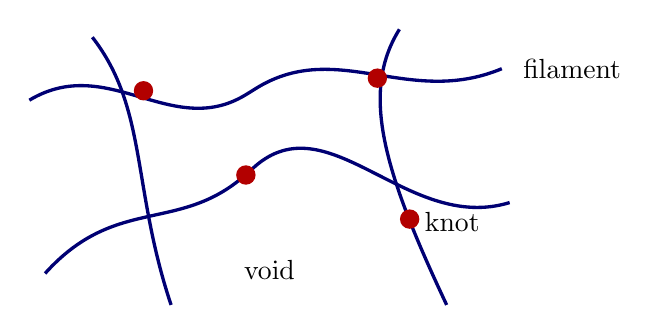
\begin{tikzpicture}[x=1cm,y=1cm]
  \draw[rounded corners=2pt,very thick,blue!45!black]
    (0.2,2.7) .. controls (1.2,3.3) and (2.0,2.2) .. (3.0,2.8)
    .. controls (4.1,3.5) and (5.0,2.6) .. (6.2,3.1);
  \draw[rounded corners=2pt,very thick,blue!45!black]
    (0.4,0.5) .. controls (1.3,1.5) and (2.1,1.0) .. (3.0,1.8)
    .. controls (4.0,2.7) and (5.0,1.0) .. (6.3,1.4);
  \draw[rounded corners=2pt,very thick,blue!45!black]
    (1.0,3.5) .. controls (1.7,2.6) and (1.5,1.6) .. (2.0,0.1);
  \draw[rounded corners=2pt,very thick,blue!45!black]
    (4.9,3.6) .. controls (4.4,2.8) and (4.7,1.8) .. (5.5,0.1);
  \fill[red!70!black] (1.65,2.82) circle (3.5pt);
  \fill[red!70!black] (4.62,2.98) circle (3.5pt);
  \fill[red!70!black] (2.95,1.75) circle (3.5pt);
  \fill[red!70!black] (5.03,1.19) circle (3.5pt);
  \node[align=center] at (3.25,0.55) {void};
  \node[right] at (6.35,3.1) {filament};
  \node[right] at (5.1,1.15) {knot};
\end{tikzpicture}
\caption{Наглядная двумерная аналогия сети каустик: линейные концентрации окружают пустоты и сходятся в более ярких узлах. В трех измерениях первичные складки представляют собой поверхности, пересечения которых образуют филаменты и узлы.}
\label{fig:c09-caustic-network}
\end{figure}

Построение без учета сил не заменяет космологическую теорию возмущений. Гравитация имеет решающее значение для роста контраста плотности, формирования гало и галактик, а также нелинейных структур. Эта модель-игрушка выделяет один устойчивый геометрический факт: слегка меняющийся начальный поток естественным образом складывается и концентрируется. Можно было бы также включить малые начальные вариации плотности, не изменяя основного аргумента, основанного на якобиане.

Следовательно, мы скорее перенесли загадку, чем устранили ее. Инфляция была введена затем, чтобы растянуть область, пока она не станет чрезвычайно плоской и однородной. Расчет каустик предполагает начальное поле крошечных вариаций скорости. Откуда взялась эта неоднородная затравка? В следующей лекции речь пойдет о квантовых флуктуациях полей во время инфляции и о том, как они становятся начальными условиями для последующей космической паутины.

\section{Что установлено этим рассуждением}

Однородное скалярное поле ведет себя как координата, движущаяся в потенциале \(V(\phi)\). В фиксированном объеме оно подчиняется уравнению \(\ddot\phi=-V'(\phi)\). В расширяющемся сопутствующем объеме физический объем \(a^3\) входит в действие и приводит к
\[
\ddot\phi+3H\dot\phi=-V'(\phi).
\]
Хаббловское трение может удерживать поле в режиме медленного установившегося движения на высоком, пологом потенциале. Тогда его кинетическая энергия становится пренебрежимо малой, потенциальная энергия поддерживает \(H\) почти постоянным, а \(a(t)\) растет приблизительно экспоненциально.

Расширение разрежает нежелательные монополи, сглаживает геометрию и сводит кривизну к нулю. Однако инфляция должна закончиться. Поле покидает плато, осциллирует и передает свою энергию горячим частицам на стадии разогрева. Несколько вопросов остаются открытыми: форма потенциала, природа и начальное состояние инфлатона, его константы связи, отвечающие за разогрев, и крошечная энергия вакуума, наблюдаемая сегодня.

Успех инфляции порождает последний вопрос. В идеально сглаженной Вселенной не было бы галактик. Каустическое отображение
\[
y=x+v(x)t,
\qquad
\frac{dn}{dy}=\frac{1}{1+v'(x)t}
\]
показывает, как крошечные вариации в начальном потоке могут порождать резкие поверхности, филаменты и узлы. Оно не объясняет происхождение этих вариаций. Теперь рассуждение обращается к их квантовому происхождению.
